% Ubah judul dan label berikut sesuai dengan yang diinginkan.
\section{Result}
\label{sec:result}

% Ubah paragraf-paragraf pada bagian ini sesuai dengan yang diinginkan.
\subsection{LSTM hyperparameter combinations}
\label{subsec:lstm-hyperparameter-combinations}
\par Figure \ref{fig:lstm-tuning} shows how the F1 score on validation data varies with the hyperparameter combinations used in Table \ref{tab: hyperparameter-lstm}. Even though the difference is insignificant, the highest F1 score is achieved when using 128 dimensions of embedding and two hidden layers of uni-directional LSTM with 32 units each, as illustrated in Figure \ref{fig:best-model-architecture}. Referring to Figure \ref{fig:lstm-performance-per-epoch}, the performance of LSTM on train and validation data is similar. This means that the model can generalize well to new data and is not overfitting or underfitting the training data.

\begin{figure}[!h]
  \centering
  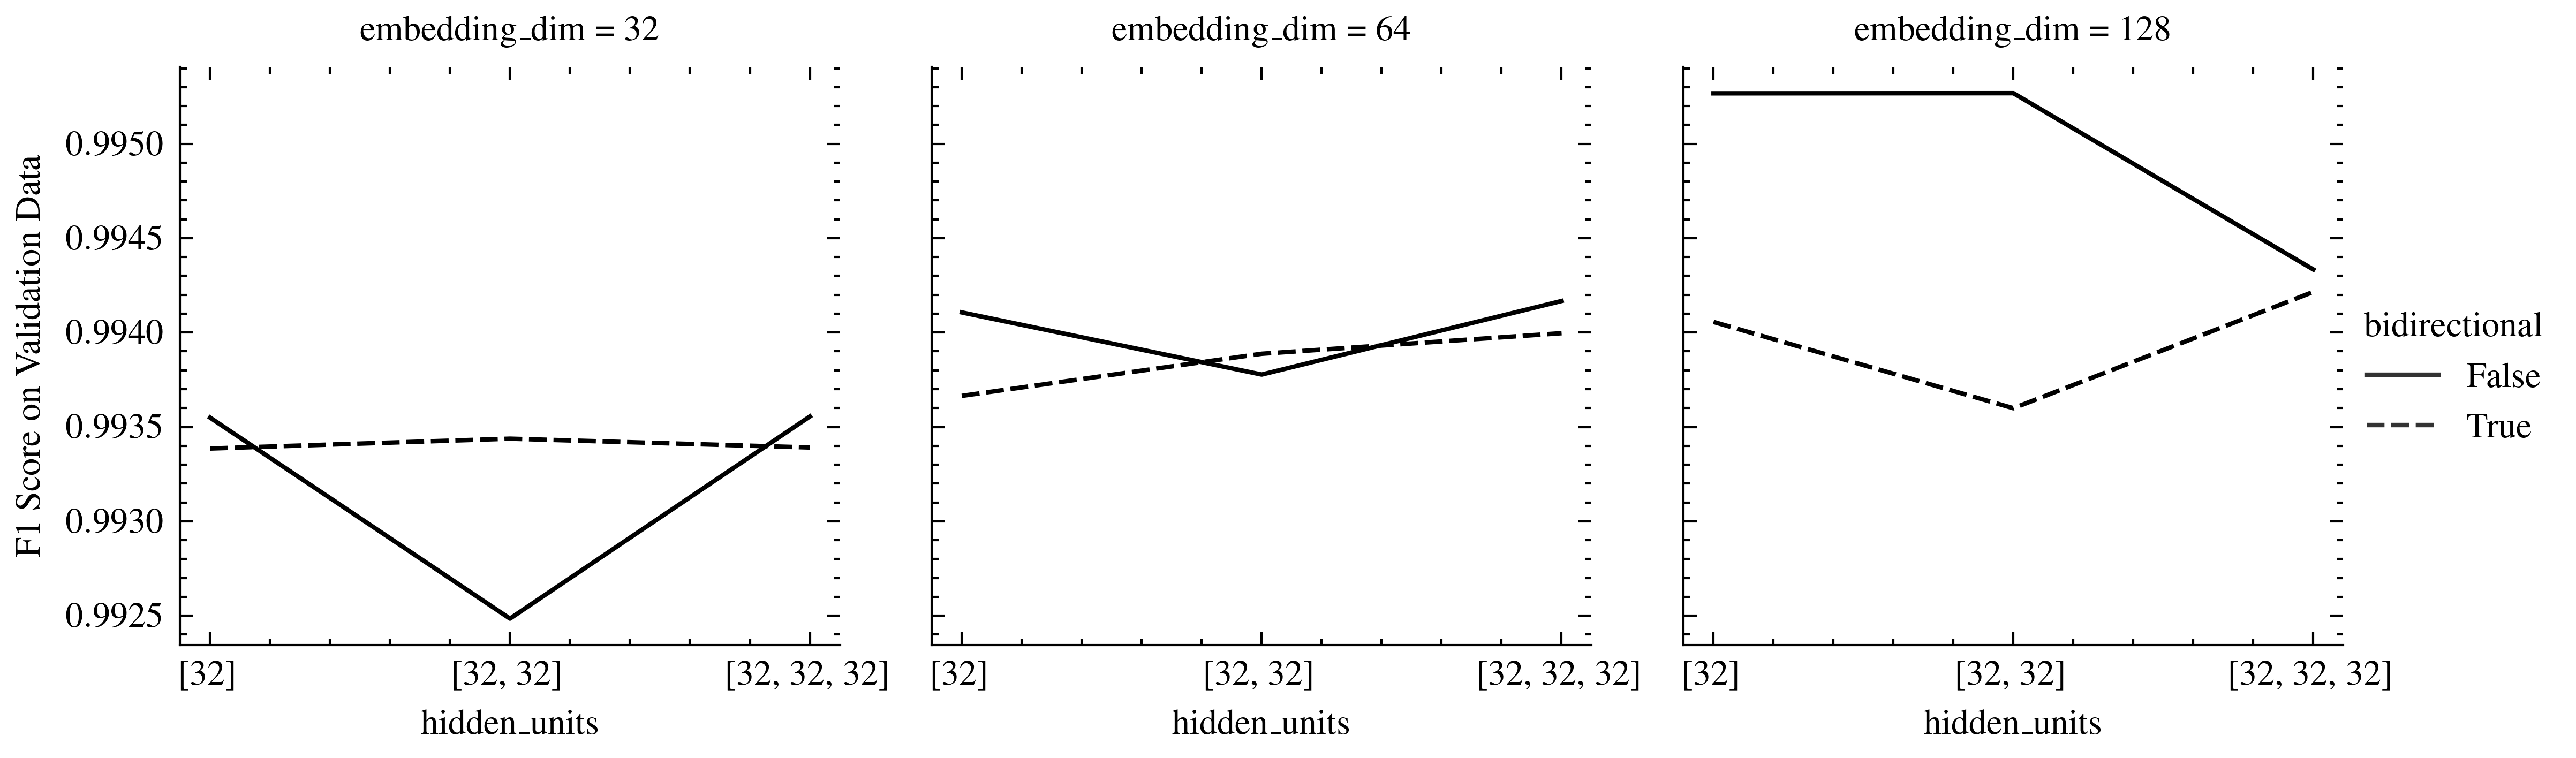
\includegraphics[width=.5\textwidth]{image/lstm_hyperparameter_tuning.png}
  \caption{LSTM hyperparameter combinations result}
  \label{fig:lstm-tuning}
\end{figure}

\begin{figure}[!h]
  \centering
  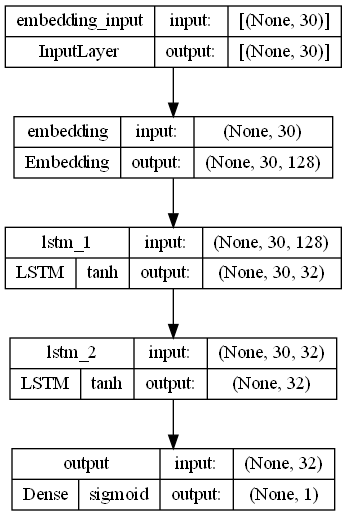
\includegraphics[width=.26\textwidth]{image/lstm_best_model_architecture.png}
  \caption{Best model architecture for LSTM}
  \label{fig:best-model-architecture}
\end{figure}

\begin{figure}[!h]
  \centering
  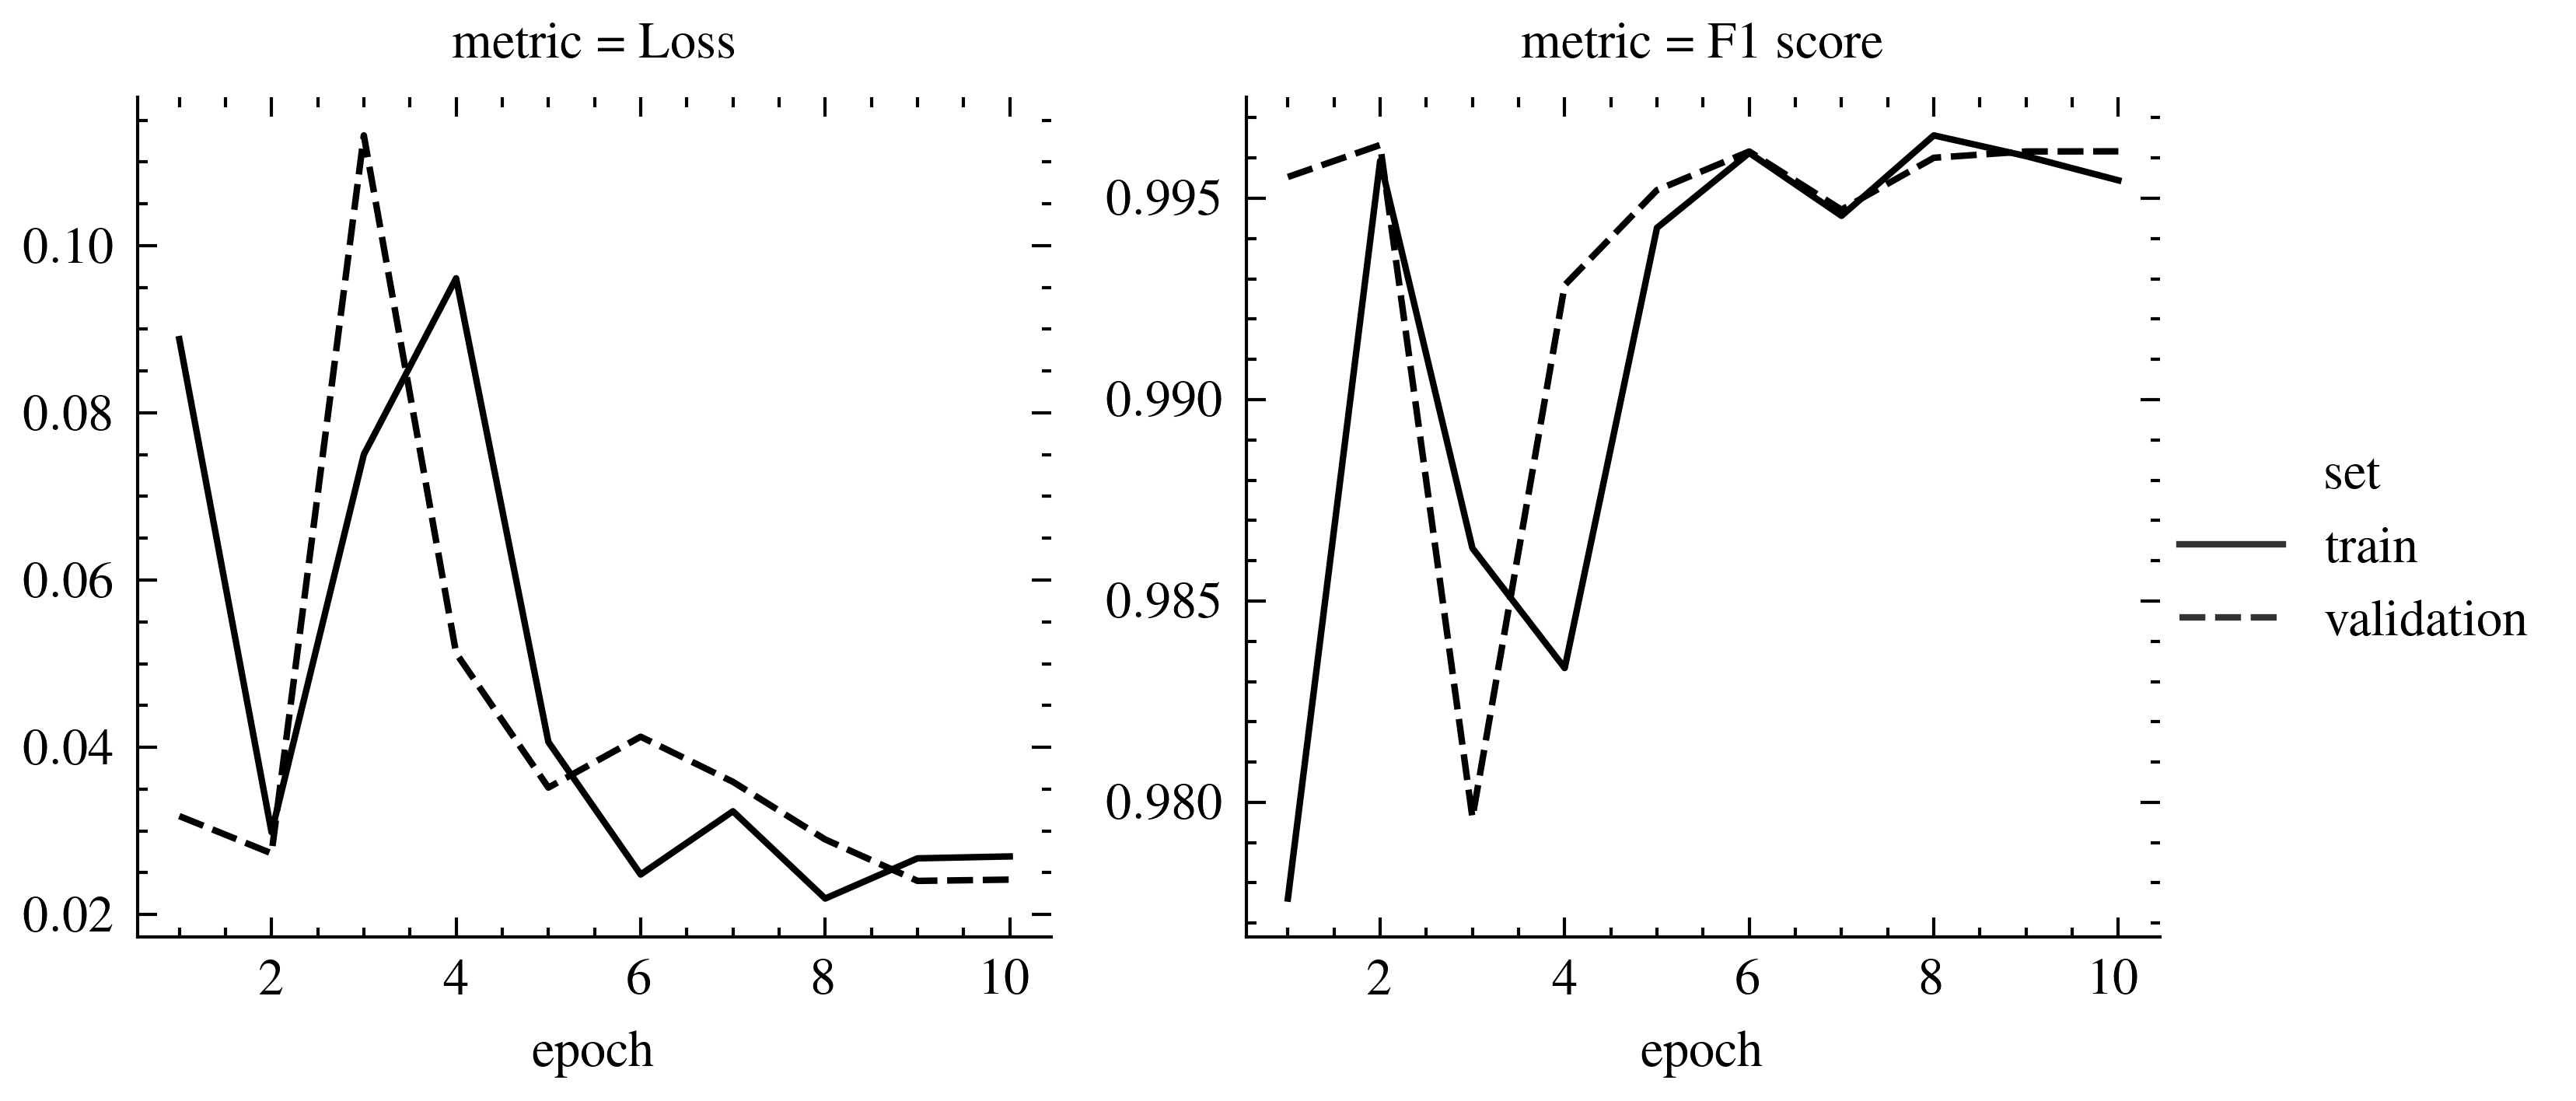
\includegraphics[width=.5\textwidth]{image/lstm_best_model_performance_per_epoch_without_acc.png}
  \caption{Performance per epoch for LSTM}
  \label{fig:lstm-performance-per-epoch}
\end{figure}

\subsection{Comparison with machine learning algorithms}
\label{subsec:comparison-with-machine-learning}
\par The LSTM model in Figure \ref{fig:best-model-architecture} is then compared with the ten classical machine learning algorithms in terms of F1 score and prediction time, measured in milliseconds per query. In Figure \ref{fig:ml_and_lstm_time_vs_f1}, the model in the lower-right region is preferred since it has a higher F1 score and faster prediction time. In the end, we still chose LSTM as our model in the prediction phase since it achieves the best F1 score and the prediction time is relatively fast compared to other algorithms.

\begin{figure}[!h]
  \centering
  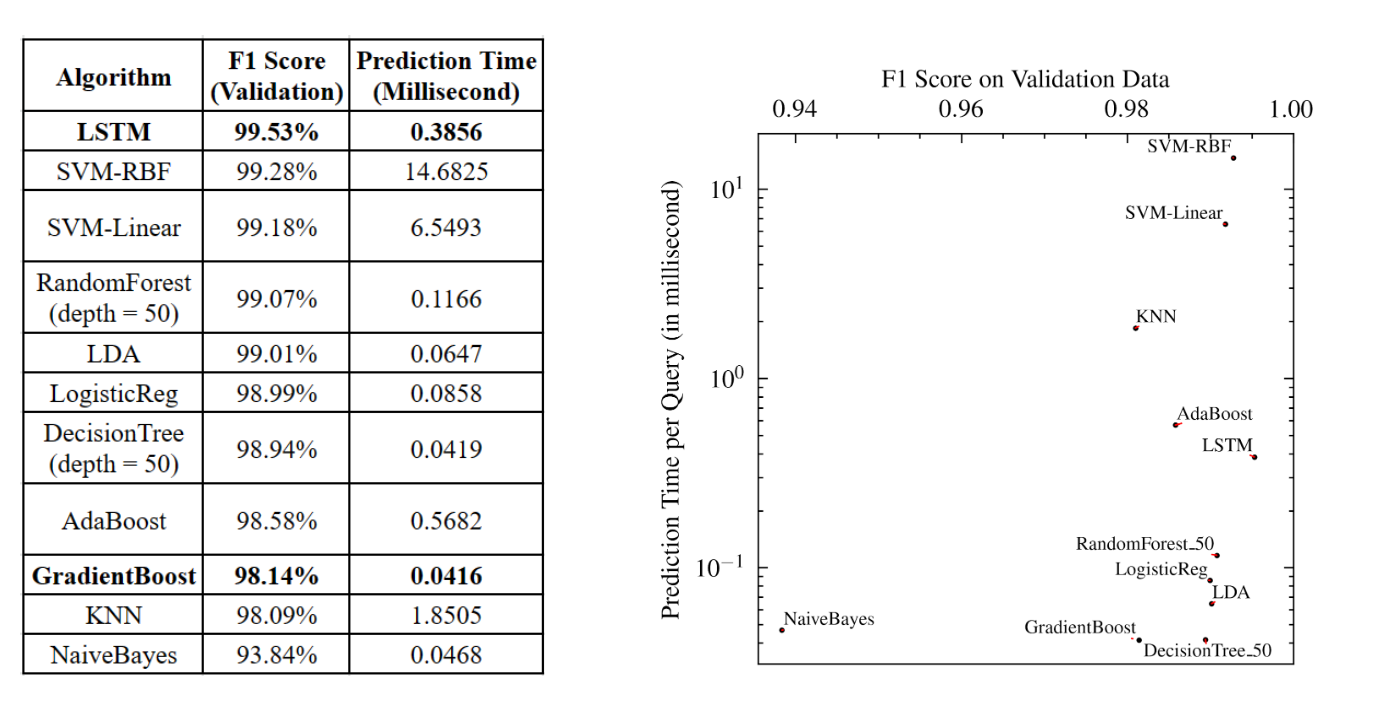
\includegraphics[width=.5 \textwidth]{image/ml-compare.png}
  \caption{Prediction time versus F1 score on 11 different algorithms}
  \label{fig:ml_and_lstm_time_vs_f1}
\end{figure}

\subsection{Comparison of the one-step and two-step approach}
\label{subsec:comparison-two-step}
\par Table \ref{tab: one-step-vs-two-step} shows the comparison between our one-step and two-step approaches. The one-step approach applies only keyword filtering or model prediction separately. Meanwhile, the two-step approach is done by combining both approaches. The keyword filtering using a blacklist help the model prediction to increase the final F1 score on test data by 0.11\%. Although insignificant, it still proves that using a two-step approach is better than only using one of either approach.

\begin{table*}[!htp]\centering
\caption{One-step versus two-step approach}\label{tab: one-step-vs-two-step}
\scriptsize
\begin{tabular}{lrrrrr}\toprule
\multirow{}{}{\textbf{Prediction Approach}} &\multicolumn{2}{c}{\textbf{Accuracy}} &\multicolumn{2}{c}{\textbf{F1 Score}} \\\cmidrule{2-5}
&\textbf{Train} &\textbf{Test} &\textbf{Train} &\textbf{Test} \\\midrule
Only model prediction &99.65\% &99.27\% &99.52\% &99.01\% \\
Only keyword filtering &63.29\% &63.31\% &0.59\% &0.61\% \\
Two-step prevention (Proposed method) &99.7\% (+0.05\%) &99.35\% (+0.08\%) &99.59\% (+0.07\%) &99.12\% (+0.11\%) \\
\bottomrule
\end{tabular}
\end{table*}

\subsection{Comparison with related work}
\label{subsec:comparison-two-step}

\par As shown in Table \ref{tab:comparison-with-related-works }, our proposed design demonstrates strong predictive capabilities and is competitive with state-of-the-art models like LSTM and CNN. While our proposed approach does have slightly lower performance than the LSTM in \cite{8877739}, it's worth noting that the LSTM in \cite{8877739} (DS5) was trained on a dataset with a different ratio of positive to negative samples (5:5 ratio). Specifically, SQLi detection performs best when the ratio of positive to negative samples is between 4:5 and 5:5, and its performance decreases as the proportion of positive samples increases. For the CNN Comparison, despite the slight disadvantage in performance, our proposed design still outperforms the CNN model in \cite{8616823} by a factor of 10 in terms of prediction time.

\begin{table}[!htp]\centering
\caption{Comparison with related work}\label{tab:comparison-with-related-works }
\scriptsize
\begin{tabular}{lrrrrr}\toprule
\multirow{}{}{\textbf{Prediction Approach}} &\multicolumn{2}{c}{\textbf{Accuracy}} &\multicolumn{2}{c}{\textbf{F1 Score}} \\\cmidrule{2-5}
&\textbf{Train} &\textbf{Test} &\textbf{Train} &\textbf{Test} \\\midrule
Dense Neural Network \cite{SQLiDataset} &- &97.73\% &- &96.36\% \\
Ensemble Boosted Trees \cite{8959617} &93.70\% &- &- &- \\
Support Vector Machine \cite{7987433} &- &98.60\% &- &98.50\% \\
LSTM (DS1) \cite{8877739} &- &93.74\% & &92.99\% \\
LSTM (DS5) \cite{8877739} &- &99.58\% &- &99.76\% \\
CNN \cite{8616823} &- &99.93\% &- &99.95\% \\
\textbf{Two-step prevention (ours)} & \textbf{99.70\%} & \textbf{99.35\%} & \textbf{99.59\%} & \textbf{99.12\%} \\
\bottomrule
\end{tabular}
\end{table}